\documentclass[a4paper]{article}

\usepackage{tikz}
\usetikzlibrary{bayesnet}
\title{Time-Aware Ailment Topic Aspect Model}
% \author{Sumit Sidana}

\begin{document}

\maketitle

  % Define nodes
  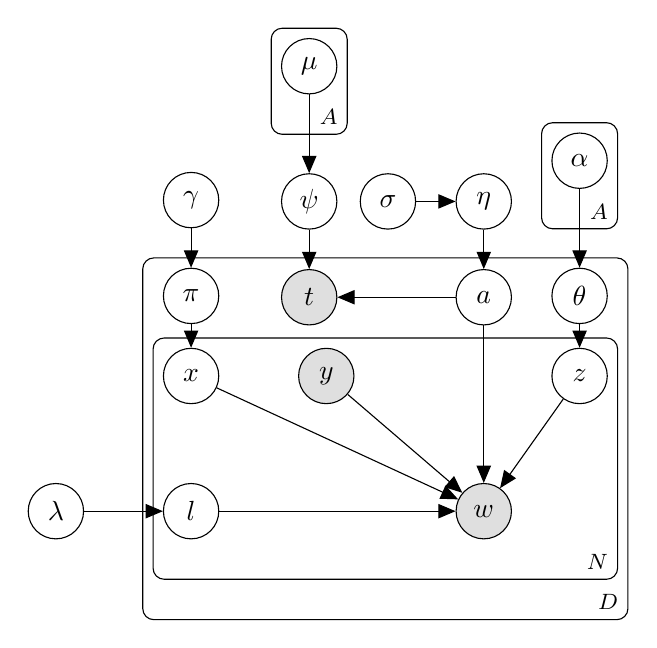
\begin{tikzpicture}[x=1.7cm,y=4.8cm]
  % Nodes

  \node[obs]                   (word)      {$w$} ; %
  \node[latent, left=3cm of word] (background) {$l$};
  \node[latent, above=1cm of background] (route) {$x$};
  \node[obs, right=1cm of route]    (aspect)      {$y$} ; %
  \node[latent, right=2.5cm of aspect]    (topic)  {$z$}; %
  \node[latent, above=2cm of word] (ailment) {$a$};
  \node[obs, left=1.5cm of ailment] (timestamp) {$t$};
  \node[latent,above=0.3cm of topic] (theta){$\theta$};
  \node[latent,above=0.3cm of route] (pi){$\pi$};
  \node[latent,left=1cm of background](lambda){$\lambda$};
  \node[latent,above=0.5cm of ailment](eta){$\eta$};
  \node[latent,left=0.5cm of eta](sigma){$\sigma$};
  \node[latent,above=0.5cm of pi](gamma){$\gamma$};
  \node[latent,above=0.5cm of timestamp](psi){$\psi$};
  \node[latent,above=1cm of psi](mu){$\mu$};
  \node[latent,above=1cm of theta](alpha){$\alpha$};
 
%   \node[const, above=of topic] (atheta) {$\alpha_\theta$};
  
\edge {background,route,aspect,topic,ailment} {word} ;
\edge {ailment}{timestamp}
\edge {theta}{topic}
\edge {pi}{route}
\edge {lambda}{background}
\edge {eta}{ailment}
\edge {sigma}{eta}
\edge {gamma}{pi}
\edge {psi}{timestamp}
\edge {mu}{psi}
\edge {alpha}{theta}

  \plate {plate1} {(word)(background)(route)(aspect)(topic)} {$N$} ;
  \plate {} {(word)(background)(route)(aspect)(topic)(ailment)(timestamp)(theta)(pi)(plate1)}{$D$};
  \plate {} {(mu)}{$A$}
  \plate {} {(alpha)}{$A$}
  % Factors
%   \factor[above=of X]     {X-f}     {Multi} {} {} ; %
%   \factor[above=of T]     {T-f}     {left:Multi} {} {} ; %
%   \factor[above=of theta] {theta-f} {left:Dir} {} {} ; %

  % More nodes
%   \node[latent, right=of X-f] (phi)  {$\phi$}; %
%   \node[const, above=of phi]  (aphi) {$\alpha_\phi$}; %

%   \factor[above=of phi] {phi-f} {right:Dir} {} {} ; %

%   \factoredge {theta}  {T-f}     {T} ; %
%   \factoredge {atheta} {theta-f} {theta} ; %
%   \factoredge {phi}    {X-f}     {X} ; %
%   \factoredge {aphi}   {phi-f}   {phi} ; %
% 
%   \gate {X-gate} {(X-f)(X-f-caption)} {T}

%   \plate {plate1} { %
%     (X)(X-gate) %
%     (T)(T-f)(T-f-caption) %
%   } {$\forall 1 \leq i \leq n_d$}; %
%   \plate {} { %
%     (plate1) %
%     (theta)(theta-f)(theta-f-caption) %
%   } {$\forall d \in \mathcal{D}$} ; %
%   \plate {} { %
%     (phi)(phi-f)(phi-f-caption) %
%   } {$\forall t \in \mathcal{T}$} ; %
  \end{tikzpicture}
% TikZ examples for graphical models (Bayesian networks) and directed
% factor graphs \cite{Dietz:2010}.
\end{document}
